\chapter{Badanie}

W niniejszej pracy przeprowadziłem metaanalizę na zbiorze danych pozyskanych z~repozytorium zbiorów danych do uczenia maszynowego UCI \cite{Dua:2021}.
Większość kroków w~badaniu (poza pozyskaniem danych) jest uniwersalnych i~można je zastosować dla innych zbiorów danych o~podobnej zawartości.
W tym rozdziale w~nawiasach kwadratowych umieszczam angielskie nazwy używanych pojęć, pod jakimi znajdują się w~analizowanym źródłowym zbiorze danych.

\section{Badanie}

Przeprowadzone badanie to analiza metadanych o~zbiorach danych zawartych w~repozytorium UCI \cite{Dua:2021}.
Serwis ten posiada informacje na temat wielu przekazanych im zbiorów danych, rejestrując jawnie informacje o~ich cechach.
Cechy te to:

\begin{itemize}
  \item Cechy zbioru danych [\emph{Data Set Characteristics}] \\
        Posiada informacje o~charakterystyce danego zbioru danych.
        Zawiera, czy zbiór jest wielowymiarowy [\emph{Multivariate}], czy jednowymiarowy [\emph{Univariate}]\footnotemark.
        \footnotetext{Statystyka wielowymiarowa zajmuje się badaniem i~obserwacją wielu zmiennych wyjścia (metryk) na raz. Statystyka jednowymiarowa bada wyłącznie zachowanie jednej zmiennej w~zbiorze.}
        Pojawia się również informacja czy zbiór ma charakter tekstowy [\emph{Text}], czy może są to dane szeregu czasowego [\emph{Time-Series}].

  \item Cechy atrybutów [\emph{Attribute Characteristics}] \\
        Zawiera informacje na temat typów atrybutów danych w~zbiorze.
        Sprecyzowane są trzy wartości: zawartość danych kategorialnych [\emph{Categorical}], liczb całkowitych [\emph{Integer}] oraz rzeczywistych [\emph{Real}].

  \item Powiązane zadania [\emph{Associated Tasks}] \\
        Zawiera informacje na temat głównych zadań, dla których dany zbiór jest przeznaczony.
        Może być to klasyfikacja [\emph{Classification}], regresja [\emph{Regression}] czy odnajdywanie powiązań przyczynowych [\emph{Causal-Discovery}].

  \item Liczba instancji [\emph{Number of Instances}] \\
        Ilość krotek (rekordów) danych zawartych w~zbiorze.
        Jeśli zbiór ma postać tabelaryczną, będzie to ilość zawartych w~nim wierszy.

  \item Liczba atrybutów [\emph{Number of Attributes}] \\
        Ilość cech, na temat których w~rekordach zawarte są dane.
        Jeśli zbiór ma postać tabelaryczną, będzie to ilość zawartych w~nim kolumn.

  \item Brakujące wartości [\emph{Missing Values}] \\
        Zawiera informację, czy w~zbiorze danych pojawiają się brakujące wartości.

  \item Obszar [\emph{Area}] \\
        Zawiera informację na temat przynależności zbioru danych do jednej z~ogólnie pojętych dziedzin tematycznych.
        Najczęściej pojawiające się tu wartości to dziedzina społeczna [\emph{Social}], fizyka [\emph{Physical}], tematy powiązane z~komputerami [\emph{Computer}] oraz życie [\emph{Life}].

  \item Data dotacji [\emph{Date Donated}] \\
        Data przekazania zbioru danych przez jego właściciela czy autora administracji repozytorium UCI.

  \item Ilość wyświetleń [\emph{Number of Web Hits}] \\
        Liczba wszystkich osób odwiedzających stronę zawierającą zbiór danych.

\end{itemize}

\subsection{Pozyskanie danych}

Repozytorium UCI nie posiada API pozwalającego na dostęp do zawartych w~nim danych.
Aby uzyskać dane w~nim zawarte napisałem więc w~języku Python program typu scraper.

Część ze zbiorów danych na stronie posiada sekcję \emph{Papers That Cite This Data Set}.
Pierwotnie scraper miał liczyć wymienione tam prace i~zapisać jako dodatkowy atrybut generowanego zbioru danych: liczbę cytacji [\emph{Number of Citations}].
Jak się okazuje, listowanie prac cytujących dany zbiór wykonywane było automatycznie z~pomocą portalu \emph{Rexa.info}.
Niestety, portal ten już nie istnieje i~bardzo trudno znaleźć o~nim informacje.
Co jest jednak pewne, to że w~wygenerowanym zbiorze danych ostatni rekord, który posiada przynajmniej jedną cytację, ma datę dotacji w~roku 2002.
Najprawdopodobniej mniej więcej w~tamtym okresie portal \emph{Rexa.info} przestał zbierać informacje na temat cytacji zbiorów danych zawartych w~repozytorium.
Tak czy inaczej, atrybut ten zebrany w~ten sposób -- mimo, że bardzo atrakcyjny jako metryka metaanalizy -- nie nadaje się do tego badania z~powodu jego bardzo ograniczonego zasięgu.
Stąd w~finalnej wersji zbioru danych został on pominięty.

Program scrapera został podzielony na dwie części, pierwsza odpowiedzialna za pobranie odpowiednich danych z~sieci i~zapisanie ich do pliku, a~druga za przetworzenie powstałego pliku i~dodanie do niego dodatkowych kolumn przydatnych przy analizie.
Część pierwsza sama również działa dwuetapowo.
Najpierw pobiera ze strony \url{http://archive.ics.uci.edu/ml/datasets} listę linków do poszczególnych zbiorów danych i~zapisuje ją do pliku.
Następnie wczytuje ten plik z~listą linków i~kolejno otwiera dane linki prowadzące do podstron konkretnych zbiorów danych, skąd pobiera szczegółowe informacje na temat tego zbioru.
Taki podział pozwala na ręczną ingerencję w~linki pobrane ze strony głównej, co okazuje się w~tym przypadku być przydatne.
Pierwotnie pobranych linków było dokładnie 559, jednak 5~z nich jest uszkodzonych.
Ręczne wyszukanie zbiorów danych o~podanej nazwie w~internecie pozwoliło na odnalezienie trzech z~nich.
Po poprawieniu linków do nich prowadzących w~pliku i~usunięciu tych, których nie udało się odnaleźć, powstał plik zawierający dokładnie 557 linków do podstron zbiorów danych w~repozytorium.
Taki poprawiony plik następnie druga część scrapera wykorzystała do wygenerowania zbioru składającego się z~informacji o~tych właśnie 557 zbiorach danych.

Druga część scrapera wzbogaca powstały zbiór danych w~dwa dodatkowe atrybuty wyliczeniowe.
Pierwszym jest ilość dni, jaką dany zbiór jest dostępny w~repozytorium [\emph{Days Available}].
Otrzymywany on jest poprzez obliczenie różnicy między datą uruchomienia scrapera a~datą dotacji zbioru do repozytorium.
Następnie z~użyciem tego pola skrypt dodaje jeszcze jedną kolumnę zawierającą liczbę wyświetleń danego zbioru na dzień [\emph{Number of Web Hits per Day}] poprzez podzielenie liczby wyświetleń przez liczbę dni dostępności zbioru.

\subsection{Przeprowadzenie analizy}

Za metrykę zbioru danych, względem której przeprowadzam analizę, obrałem ilość wyświetleń danego zbioru na dzień.
Wartość ta jest znormalizowana czasowo, co pozwala na uwzględnienie jej jako odzwierciedlenia popularności zbioru.

Analiza została przeprowadzona przy użyciu portalu \emph{Azure Machine Learning Studio (classic)}.
Utworzyłem 6~eksperymentów wykorzystujący wygenerowany przez scrapera zbiór danych.
Jeden z~eksperymentów bada zależności między atrybutami numerycznymi, a~pozostałe 5~dzielą zbiór na podzbiory bazując na różnych danych kategorialnych oraz liczą statystyki związane z~wyświetleniami dla każdego z~nich.

W Azure ML moduł odpowiedzialny za badanie zależności przy kolumnach numerycznych bazuje na wyliczeniu współczynnika korelacji liniowej Pearsona.
Zestawia on atrybuty na zasadzie ``każdy z~każdym'' i~liczy korelację liniową między nimi.
W ten sposób powstaje macierz korelacji, która na przekątnej będzie miała wartości \( 1~\) (każdy atrybut zestawiony jest również ze sobą, jest to więc autokorelacja).
Współczynnik korelacji mieści się w~przedziale domkniętym \( [-1, 1] \).
Wartość ujemna mówi, że gdy jeden atrybut rośnie, drugi maleje, a~dodatnia, że oba atrybuty wspólnie rosną i~maleją.
Dodatkowo wartość bezwzględna współczynnika opisuje, jak silna jest zależność pomiędzy atrybutami.

5 pozostałych eksperymentów badało wpływ danych kategorialnych na obraną metrykę zbioru.
W każdym z~nich zbiór został podzielony na kilka podzbiorów poprzez rozbicie jednej z~kolumn kategorialnych na podkategorie, a~następnie wyliczenie podstawowych statystyk numerycznych kolumny z~metryką każdego z~nich.
Następnie na podstawie tych statystyk są wygenerowane wykresy słupkowe.
Przeprowadzone eksperymenty objęły podziałów ze względu na:

\begin{itemize}
  \item Charakterystykę zbioru danych [\emph{Data Set Characteristics}] \\
        W~tej kolumnie znajdowało się 12 unikatowych charakterystyk.
        Każdy rekord mógł posiadał wiele z~nich oddzielonych przecinkami.
        Przynależność do podzbioru określałem poprzez obecność słowa kluczowego w~tym atrybucie.
        Za granicę przyjęcia podzbioru do analizy ustaliłem, że musi posiadać przynajmniej 10 elementów.

  \item Charakterystykę atrybutów zbioru [\emph{Attribute Characteristics}] \\
        W~tej kolumnie znajdowały się dokładnie 3~unikatowe charakterystyki niewykluczające się wzajemnie.
        Stąd powstały 3~podzbiory na podobnej zasadzie jak wyżej.

  \item Obecność brakujących danych [\emph{Missing Values}] \\
        Tutaj utworzone zostały dokładnie dwa podzbiory: zbiory zawierające brakujące dane oraz te ich nie zawierające.

  \item Powiązane zadania [\emph{Associated Tasks}] \\
        W~tej kolumnie znajdowało się 9~unikatowych, niewykluczających się wzajemnie zadań.
        Przynależność do podzbioru określałem analogicznie jak w~eksperymencie z~charakterystykami zbioru danych, podobnie za granicę dolną przyjmując 10 elementów podzbioru.

  \item Obszar [\emph{Area}] \\
        Obszar cyberbezpieczeństwa [\emph{Computer Security}] zaliczyłem do obszaru informatyki, a~finansowy [\emph{Financial}] do danych biznesowych.
        Te obszary znacznie rzadziej pojawiały się w~uzyskanych danych (kolejno jednorazowo i~5 razy) i~ich analiza nie była możliwa a~dostępne były bliskie im szersze obszary.
        Obszar gier [\emph{Games}] również był ubogi (10 instancji) jednak nie przypasował się żadnej z~większych dziedzin, stąd wykluczyłem go z~analizy.

\end{itemize}

W badaniu posługuję się przede wszystkim medianą jako miarą tendencji centralnej analizowanych podzbiorów.
Mediana jest znacznie odporniejsza na wysoki współczynnik skośności danych oraz elementy odstające.
Na wykresach znajdą się słupki średniej (pomarańczowe) oraz mediany (jasne niebieskie) dziennych wyświetleń dla poszczególnych podzbiorów oraz dwie poziome linie będące odpowiednio ogólną średnią (czerwona) i~ogólną medianą (niebieska) dla całego zbioru.

\section{Wyniki}

\begin{center}
      \begin{table}[ht]
        \begin{tabular}{|l|rrr|}
          \hline
                              & Liczba instancji & Liczba atrybutów & Wyświetl. na dzień \\
          \hline
          Liczba instancji    & 1~               & 0.099287         & 0.126046           \\
          Liczba atrybutów    & 0.099287         & 1~               & -0.024657          \\
          Wyświetl. na dzień  & 0.126046         & -0.024657        & 1~                 \\
          \hline
        \end{tabular}
        \caption{Macierz korelacji liniowej między wartościami numerycznymi w~analizowanym zbiorze danych}
        \label{tab:correlation}
      \end{table}
    \end{center}

Tabela \ref{tab:correlation} przedstawia macierz korelacji atrybutów numerycznych zbioru.
Oprócz trywialnej autokorelacji nie pojawia się nigdzie żadna silna zależność.
Najwyższa wartość ( \( \sim 0.13 \) ) występuje pomiędzy ilością instancji w~zbiorze a~obraną metryką liczby wyświetleń na dzień.
Najniższa z~kolei ( \( \sim -0.02 \) ) zachodzi między wyświetleniami a~ilością atrybutów.
Sugerowało by to, większa liczba instancji w~zbiorze zwiększa jego popularność, natomiast liczba atrybutów na nią nie wpływa.
Korelacja ta jest jednak bardzo niska.
Takie wartości w~większości przypadków się określa po prostu jako brak korelacji.
Można z~tego wyciągnąć wniosek, że ani ilość atrybutów, ani ilość instancji nie ma wpływu na jakość i~popularność zbioru danych.

Zanim zaczniemy wyjaśniać wyniki poszczególnych eksperymentów warto zaznaczyć i~omówić ogólny trend, który się pojawił.
Konsekwentnie przy każdym podziale ze względu na różne charakterystyki i~cechy, każdy analizowany podzbiór przejawiał identyczną cechę.
Wszędzie mediana jest dużo niższa od średniej, uśredniając jest to około \( ~ 35\% \).
Pokazuje to wysoką skośność zbioru.
Jest to sytuacja podobna, jak kiedy osoba niewiarygodnie bogata wprowadza się do podmiejskiej dzielnicy i~w pojedynkę mocno zawyża średnią kapitału nie zmieniając przy tym szczególnie mediany.
Tutaj mała część zbiorów posiada liczbę wyświetleń znacznie większą i~odstającą od reszty, podnosząc tym samym średnią, jednak nie wpływając zasadniczo na medianę.

\begin{figure}[ht]
      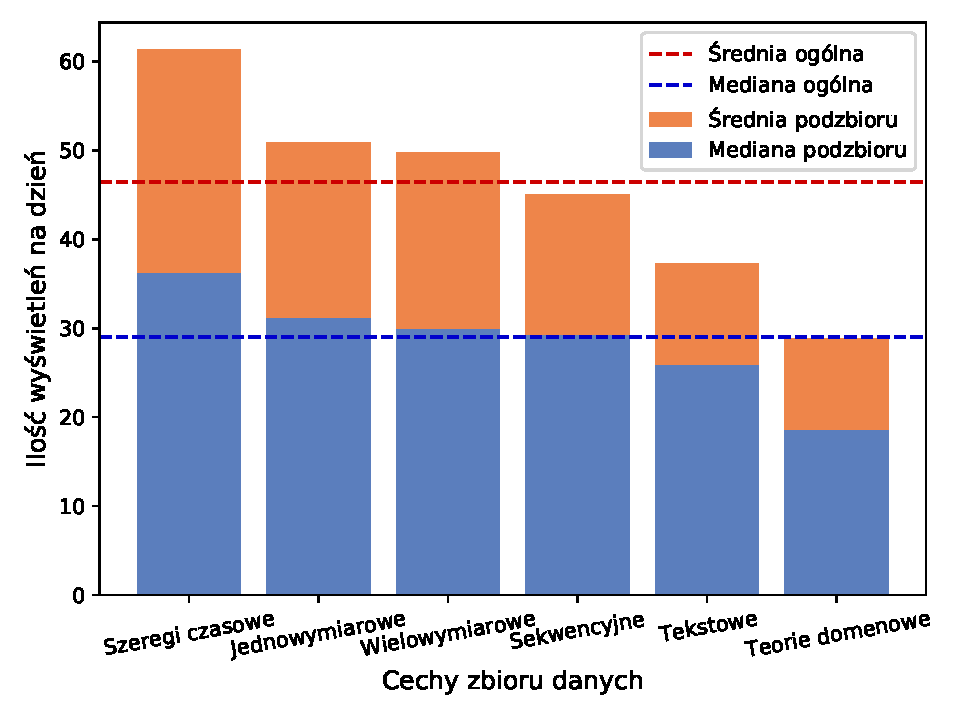
\includegraphics[width=\textwidth]{Plots/DataSetCharacteristics}
      \caption{Analiza średniej i~mediany liczby dziennych wyświetleń zbiorów danych z~podziałem względem ich charakterystyki}
      \label{fig:datasetcharacteristics}
\end{figure}

Analiza charakterystyk zbiorów danych (rysunek \ref{fig:datasetcharacteristics}) pokazuje, że najbardziej użyteczne zbiory danych zawierają szeregi czasowe [\emph{Time-Series}].
Co ciekawe, dane tekstowe są raczej mniej popularne.
Z kolei zbiory zawierające dane domenowe [\emph{Domain-Theory}] otrzymują wyraźnie najmniej zainteresowania.
Dane jednowymiarowe są również popularniejsze niż wielowymiarowe, chociaż tutaj różnica jest znacznie mniejsza.

\begin{figure}[ht]
      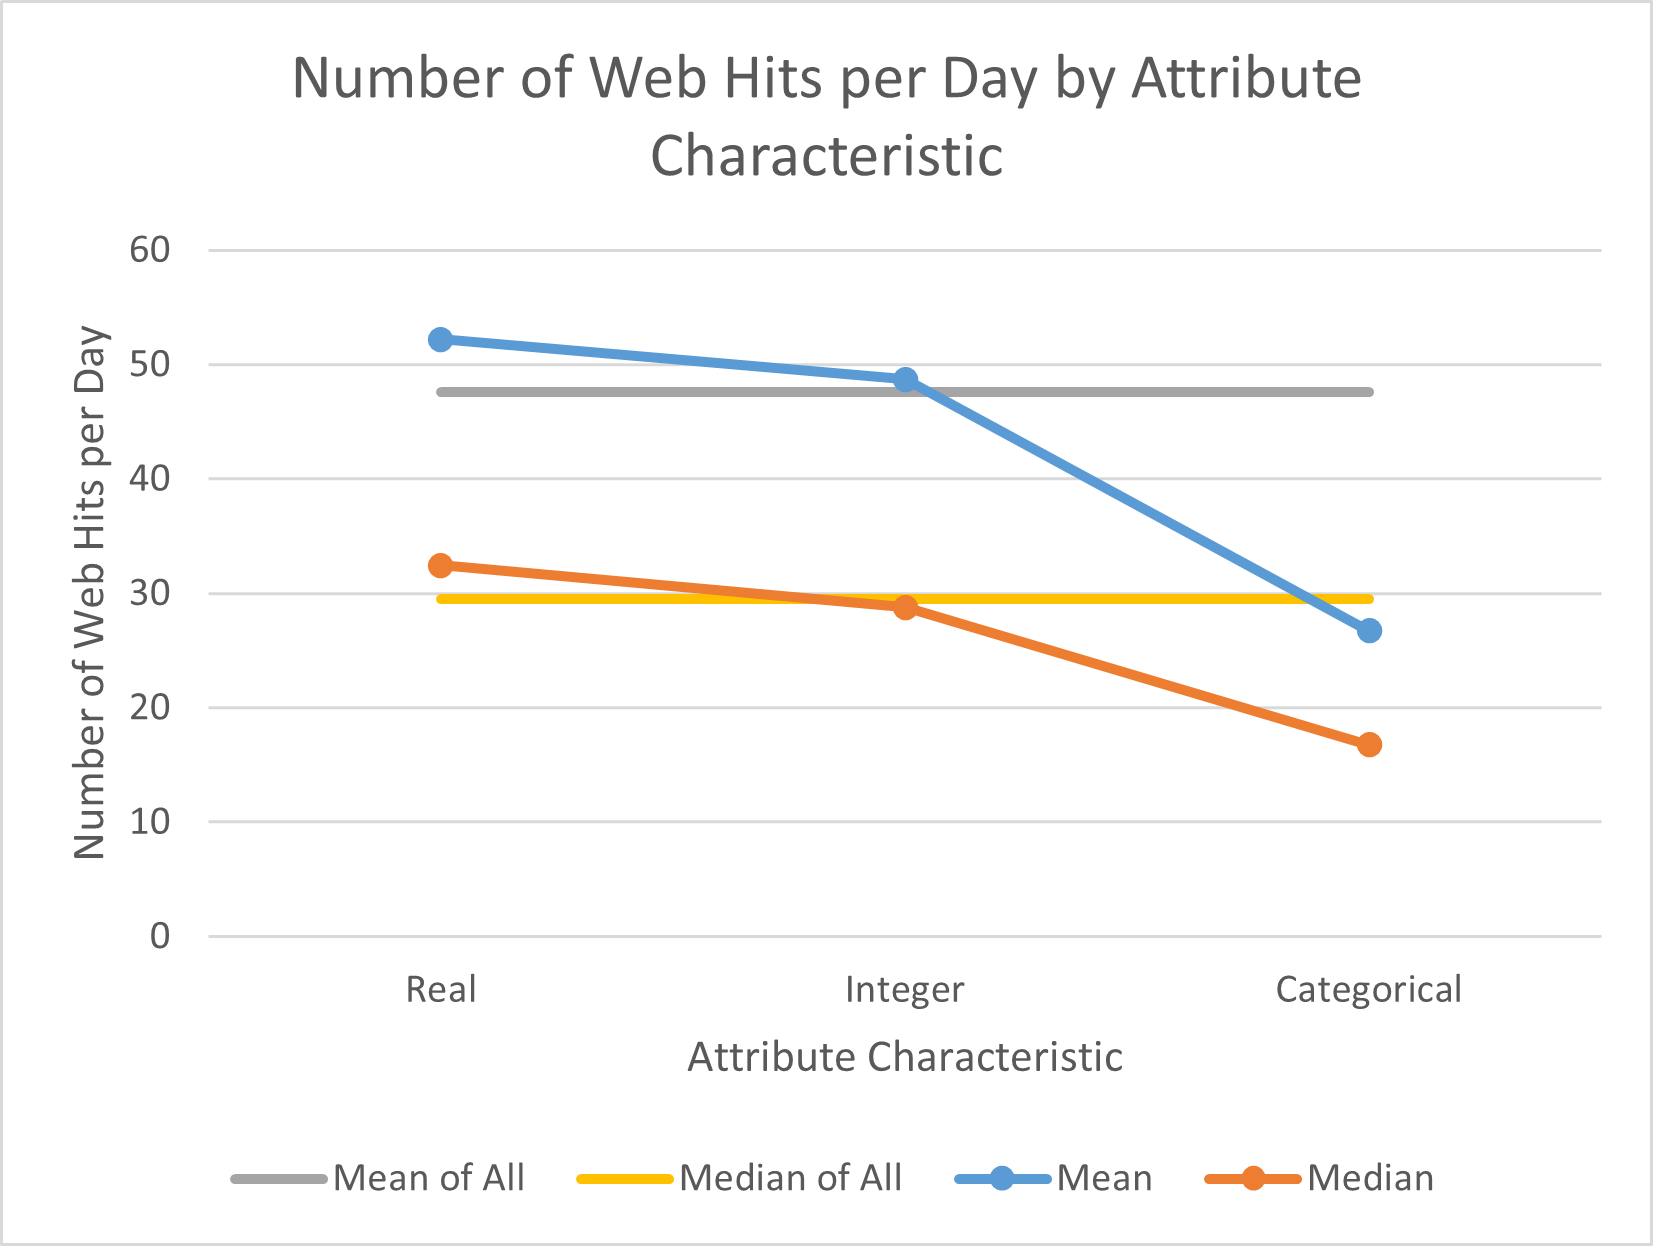
\includegraphics[width=\textwidth]{Plots/AttributeCharacteristics}
      \caption{Analiza średniej i~mediany liczby dziennych wyświetleń zbiorów danych z~podziałem względem charakterystyki zawartych w~nich atrybutów}
      \label{fig:attributecharacteristics}
\end{figure}

Analiza rodzaju danych atrybutów zawartych w~zbiorach (rysunek \ref{fig:attributecharacteristics}) pokazuje, że największym zainteresowaniem cieszą się zbiory zawierające wartości rzeczywiste.
Zawieranie liczb całkowitych jest blisko mediany ogólnej, co mówi, że ogólnie dane liczbowe są preferowane.
Dane kategorialne bowiem znacznie odbiegają od reszty i~są zdecydowanie mniej popularne.

\begin{figure}[ht]
      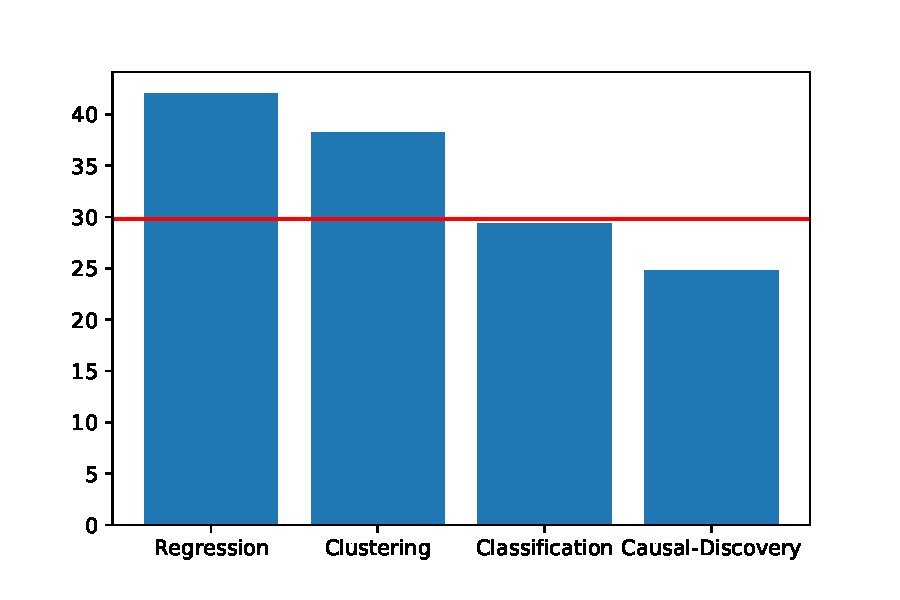
\includegraphics[width=\textwidth]{Plots/AssociatedTasks}
      \caption{Analiza średniej i~mediany liczby dziennych wyświetleń zbiorów danych z~podziałem względem powiązanych z~nimi zadań}
      \label{fig:associatedtasks}
\end{figure}

Przy analizie powiązanych zadań (rysunek \ref{fig:associatedtasks}) również można wyciągnąć dość wyraźne wnioski.
Najpopularniejsze są zbiory danych przeznaczone do przeprowadzania na nich regresji [\emph{Regression}], a~tuż za nimi te przeznaczone do analizy skupień [\emph{Clustering}].
Zbiory powiązane z~klasyfikacją [\emph{Classification}] nie odbiegają od normy, a~najmniejszym zainteresowaniem cieszą się te związane z~analizą przyczynową [\emph{Causal-Discovery}].

\begin{figure}[ht]
  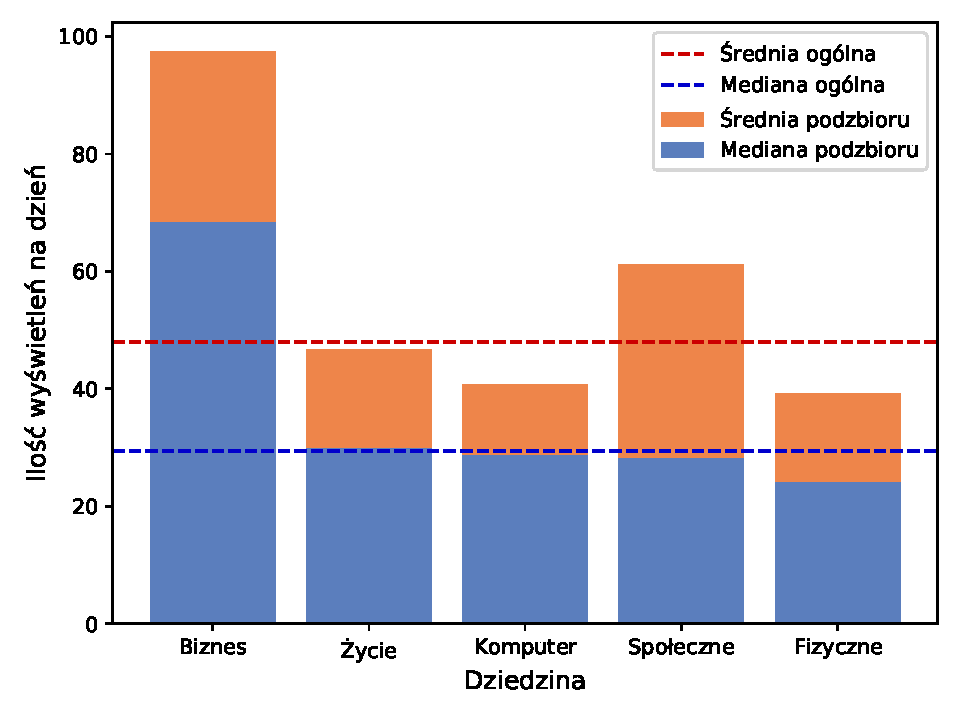
\includegraphics[width=\textwidth]{Plots/Area}
  \caption{Analiza średniej i~mediany liczby dziennych wyświetleń zbiorów danych z~podziałem względem ich dziedziny}
  \label{fig:area}
\end{figure}

Analizując bardziej semantyczną zawartość zbiorów danych, czyli ogólny obszar ich pochodzenia (rysunek \ref{fig:area}) widać, że wyraźnie najpopularniejsze są zbiory zawierające dane biznesowe.
Średnia wyświetleń zbiorów z~dziedziny społecznej również wykracza poza średnią ogólną, chociaż ich mediana już takiej tendencji nie wykazuje.
Biorąc pod uwagę ten fakt i~naturę relacji między średnią a~medianą można wyciągnąć wniosek, że w~tym obszarze kilka najczęściej odwiedzanych zbiorów mocno wybiega popularnością poza pozostałe.
95. percentyl jest równy \(215.98\), co jest prawie najwyższą wartością, jedynie za biznesem (\(303.41\)).
Z kolei 5. percentyl nie odbiega mocno od pozostałych.
W odwrotnej sytuacji są zbiory informatyczne, których 95. percentyl wynosi zaledwie \(98.93\), tylko \(75\%\) następnej najniższej wartości (obszaru fizyki).
Ta grupa ma z~kolei sporo zbiorów wyjątkowo mało popularnych.
Jednak ich mediana również się nie wyróżnia.
Jedyną grupą wyróżniającą się z~innych poza biznesową jest fizyczna.
Są one mniej popularne zarówno patrząc na średnią, jak i~medianę podzbioru.

\begin{figure}[ht]
      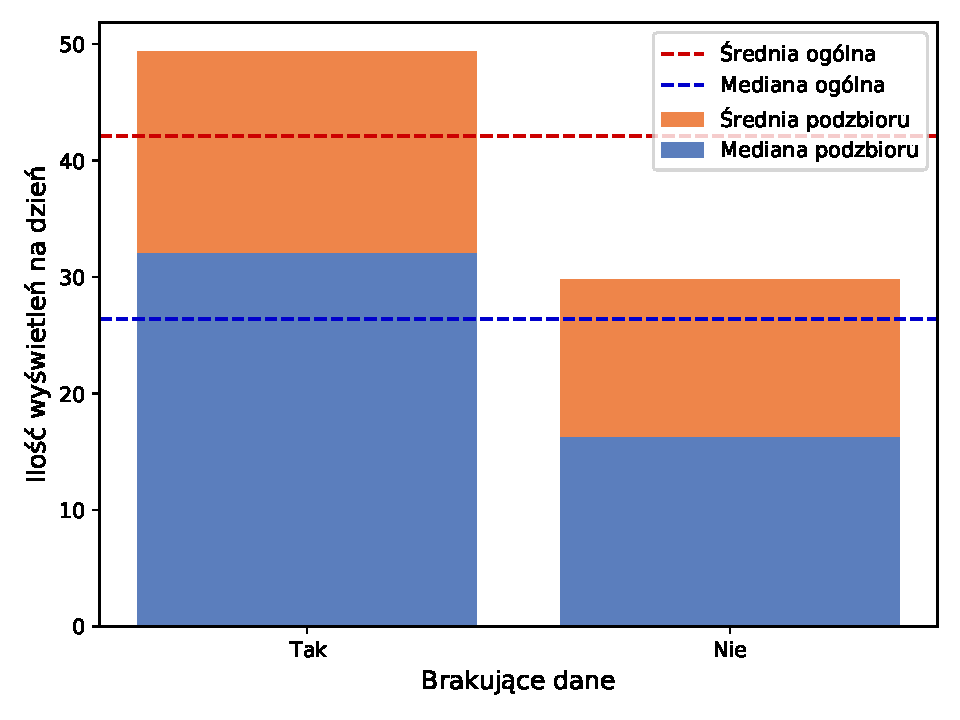
\includegraphics[width=\textwidth]{Plots/MissingValues}
      \caption{Analiza średniej i~mediany liczby dziennych wyświetleń zbiorów danych z~podziałem względem brakujących w~nich danych}
      \label{fig:missingvalues}
\end{figure}

Ciekawą sytuację przedstawia analiza brakujących danych przedstawiona na rysunku \ref{fig:missingvalues}.
Sugeruje ona, że zbiory posiadające brakujące dane przyciągają więcej osób niż te, które ich nie mają.
Jest to sprzeczne z~tym, czego można by się spodziewać zarówno intuicyjnie, jak i~biorąc pod uwagę ocenę jakości zbiorów danych.
Można to jednak wytłumaczyć biorąc pod uwagę inne cechy zbiorów.
Biorąc pod uwagę szeregi czasowe, najpopularniejszy rodzaj danych, 27 z~32 rekordów zawierających na ten temat informacje posiada brakujące dane (\(~84\%\).
Z kolei najmniej popularne dane domenowe wykazują odwrotną tendencję, gdzie \(75\%\) z~nich nie zawiera brakujących danych.

Podobna sytuacja ma miejsce gdy weźmiemy pod uwagę rodzaj atrybutów.
Zdecydowanie najpopularniejsze zbiory zawierające liczby rzeczywiste posiadają brakujące dane w~\(~72\%\) przypadków (71 z~98), a~najmniej pożądane dane kategorialne odwrotnie, nie posiadają brakujących danych w~\(55\%\) przypadków (40 z~73).
Najpopularniejszy rodzaj docelowego przeznaczenia, regresja, także wykazuje ponadprzeciętną zawartość brakujących danych (34 z~39, czyli \(~87\%\)).

Jak widać to popularniejsze kategorie danych mają dużą zawartość brakujących danych, natomiast mniej popularne mają ich znacznie mniej.
Wynikać to może z~natury charakterystyk popularniejszych zbiorów danych, które z~założenia posiadają więcej braków, jednak są one mało istotne z~perspektywy użyteczności.
Jest również możliwość, że istniejące algorytmy uzupełniania brakujących danych takie jak MICE czy PCA są na tyle dobre, że nieduże ubytki nie wpływają na jakoś uczenia czy analizy.
Tłumaczyłoby to w~szczególności różnicę między wpływem brakujących danych na liczby rzeczywiste, a~dane kategorialne, jako, że dane liczbowe można uzupełnić wspomnianymi wcześniej metodami.

\section{Dyskusja}

Otrzymane przeze mnie wyniki trudno zweryfikować poprzez zestawienie ich z~innymi podobnymi badaniami, ponieważ zgodnie z~moją wiedzą nikt nie przeprowadzał podobnych analiz w~takim kontekście.

Niektóre wyniki mogą być jednak częściowo porównane z~innymi badaniami również opartymi na samej analizie metadanych, choć w~innych kontekstach.

Moje rezultaty odnoszące się do wpływu wielkości zbioru danych (tabela \ref{tab:correlation}) pokazują, że ilość instancji oraz atrybutów nie wpływają zasadniczo na wynik analizy.
Pokrywa się to z~innymi badaniami \cite{brazdil1994characterizing}, w~których stwierdzono, że ilość danych zawartych w~zbiorze nie wpływa zasadniczo na ich wyniki związane z~aplikowalnością algorytmów uczenia maszynowego.

Z kolei wpływ brakujących danych na atrakcyjność zbioru jest sprzeczny z~innymi pracami oraz ogólną intuicją.
Moje wyniki (rysunek \ref{fig:missingvalues}) pokazują, że brakujące dane w~zbiorze nie wpływa negatywnie na jego atrakcyjność, a~nawet przeciwnie.
Inne prace \cite{yasser2011analysis} natomiast wyodrębniły brakujące dane jako jeden z~zasadniczych problemów metadanych.

Pozostałych analiz przeze mnie przeprowadzonych nie jestem w~stanie zestawić z~innymi.
Warto jednak wspomnieć o~możliwym powiązaniu między dwoma wynikami przez mnie osiągniętymi.
Z analizy charakterystyki zbiorów danych (rysunek \ref{fig:datasetcharacteristics}) można wywnioskować, że najpopularniejsze są szeregi czasowe.
Dalej, z~analizy charakterystyki atrybutów w~zbiorze (rysunek \ref{fig:attributecharacteristics}) otrzymujemy, że najpopularniejsze są zbiory zawierające liczby rzeczywiste.
Istnieje tutaj możliwe powiązanie, jako że oczywistym jest, że szeregi czasowe w~przeważającej większości zawierają liczby rzeczywiste.
Natomiast przeciwko tej tezie może mówić brak podobnego podobieństwa między szeregami czasowymi a~ilością danych, która -- jak było już wspomniane -- nie ma wpływu na atrakcyjność.
Szeregi czasowe z~reguły zawierają duże ilości danych (na przykład dane pobierane przez EEG), więc można by było spodziewać się podobnego powiązania.

Wskazane jest porównanie wyciągniętych w~tej pracy wniosków z~przyszłymi weryfikacjami, w~szczególności przeprowadzonymi z~pewniejszymi metrykami.
Takimi mogłyby być tutaj niedoszła liczba cytacji, w~których dany zbiór się pojawia, albo -- nawet lepiej -- jego wpływ na \emph{wskaźnik cytowań} (ang. \emph{impact factor}) prac go używających.
Należałoby jednak wziąć pod uwagę, że akurat te metryki skupiałyby się raczej na zastosowaniach naukowych, a~omijały komercyjne.
